\documentclass[12pt, a4paper, oneside]{ctexart}
\usepackage{amsmath, amsthm, amssymb, appendix, bm, graphicx, hyperref, mathrsfs}
\usepackage{float}
\usepackage{booktabs} 
\usepackage{caption}
\usepackage{geometry}
\geometry{margin=1in}

\title{\textbf{线性回归模型的变量选择方法}}
\author{王一鑫}
\date{\today}
\linespread{1.5}
\newtheorem{theorem}{定理}[section]
\newtheorem{definition}[theorem]{定义}
\newtheorem{lemma}[theorem]{引理}
\newtheorem{corollary}[theorem]{推论}
\newtheorem{example}[theorem]{例}
\newtheorem{proposition}[theorem]{命题}
\renewcommand{\abstractname}{\Large\textbf{摘要}}
\usepackage{listings}
\usepackage{xcolor}
\definecolor{mygreen}{rgb}{0,0.6,0}
\definecolor{mygray}{rgb}{0.5,0.5,0.5}
\definecolor{mymauve}{rgb}{0.58,0,0.82}


\lstset{numbers=left, %设置行号位置
		numberstyle=\tiny\color{mygray}, %设置行号大小
		basicstyle=\footnotesize,
		keywordstyle=\color{blue}, %设置关键字颜色
		commentstyle=\color{mygreen}, %设置注释颜色
		frame=single, %设置边框格式
		rulecolor=\color{black},
		escapeinside=``, %逃逸字符(1左面的键),用于显示中文
		%breaklines, %自动折行
		extendedchars=false, %解决代码跨页时,章节标题,页眉等汉字不显示的问题
		xleftmargin=2em,xrightmargin=2em, aboveskip=1em, %设置边距
		tabsize=2, %设置tab空格数
		showspaces=false,%不显示空格
		breaklines=true,  
		stringstyle=\color{orange}
	}


\begin{document}
	
	\maketitle
	
	\setcounter{page}{0}
	\maketitle
	\thispagestyle{empty}
	
	\begin{abstract} 
		变量选择是构建高效线性回归模型的重要环节,对于提高模型解释性和预测精度具有重要意义. 本文系统介绍了几种常用的变量选择方法,包括\textbf{岭回归}(Ridge Regression)、\textbf{Lasso回归}、\textbf{SCAD}(平滑剪切绝对偏差)方法以及\textbf{自适应Lasso}(Adaptive Lasso). 在阐述各方法数学原理的基础上,利用R语言对波士顿房价数据集进行实证分析,绘制了系数路径图与交叉验证误差图,直观展示了调节参数对模型的影响. 结果表明,不同方法在变量筛选能力、模型稀疏性和估计偏差方面各具特点,适应不同实际需求. 本文对比分析了这些方法的优劣,为实际数据建模中的变量选择提供了理论基础和实用参考.
		
		\par\textbf{关键词:}变量选择;岭回归;Lasso;SCAD;自适应Lasso \end{abstract}
	
	\newpage
	\pagenumbering{Roman}
	\setcounter{page}{1}
	\tableofcontents
	\newpage
	\setcounter{page}{1}
	\pagenumbering{arabic}
	
	\section{变量选择方法}
	
	\subsection{问题背景}
	
	“回归”的概念是1886年由英国统计学家Galton 在研究父代身高与子代身高之间的关系时提出的. 目前回归分析已成为统计学应用最为广泛的方法之一,主要用于探索和检验协变量与相应变量之间的相关关系.
	
	我们在对实际问题构建线性回归模型的过程中,可能会把对响应变量$Y$可能产生影响的协变量$X_{1}, X_{2}, \cdots X_{p}$全部引入回归方程,这会导致模型中包含了一些对$Y$影响很小的变量,出现过拟合的现象,降低了模型的预测精度,因此对协变量做变量选择是非常必要的.
	
	除了如AIC和BIC等经典的$L_{0}$惩罚变量选择方法之外,一些压缩估计方法也是重要的统计方法,例如岭回归、桥回归、Lasso、SCAD和自适应Lasso.
	
	考虑多元线性回归模型,假设对 $Y, X_1, \dots, X_p$ 进行了 $n$ 次独立的试验,得到 $n$ 组独立的观测值,即 $\{(y_i, x_{i1}, \dots, x_{ip}), i=1,\dots,n\}$. 简便起见,对协变量数据进行标准化处理,使得
	\begin{equation}
		\sum_{i=1}^{n} x_{ij} = 0, \quad \sum_{i=1}^{n} x_{ij}^2 = 1.
	\end{equation}
	
	则标准化后的数据满足
	\begin{equation}
		y_i = \beta_1 x_{i1} + \cdots + \beta_p x_{ip} + \varepsilon_i, \quad i = 1, \dots, n. \label{lm}
	\end{equation}
	
	引进矩阵记号:
	
	\[
	\bm{Y} = 
	\begin{pmatrix}
		y_1 \\
		y_2 \\
		\vdots \\
		y_n
	\end{pmatrix},
	\quad
	\bm{X} = 
	\begin{pmatrix}
		x_{11} & \cdots & x_{1p} \\
		x_{21} & \cdots & x_{2p} \\
		\vdots & \ddots & \vdots \\
		x_{n1} & \cdots & x_{np}
	\end{pmatrix},
	\quad
	\bm{\beta} = 
	\begin{pmatrix}
		\beta_1 \\
		\beta_2 \\
		\vdots \\
		\beta_p
	\end{pmatrix},
	\quad
	\bm{\varepsilon} = 
	\begin{pmatrix}
		\varepsilon_1 \\
		\varepsilon_2 \\
		\vdots \\
		\varepsilon_n
	\end{pmatrix},
	\]
	
	其中 $\bm{Y}$ 为 $n \times 1$ 的响应变量的观测向量,$\bm{X}$ 为 $n \times p$ 的已知设计矩阵,$\bm{\beta}$ 为 $p$ 维的未知参数向量,$\bm{\varepsilon}$ 为 $n \times 1$ 的随机模型误差向量。模型 \eqref{lm}写成如下矩阵形式:
	
	\begin{equation}
		\bm{Y} = \bm{X} \bm{\beta} + \bm{\varepsilon}.\label{matrixlm}
	\end{equation}
	
	
	\subsection{岭回归}
	\subsubsection{模型原理}
	岭回归(Ridge Regression),也称为Tikhonov正则化(Tikhonov Regularization),是一种专门用于处理多重共线性(特征之间高度相关)问题的线性回归改进算法. 在多重共线性的情况下,数据矩阵可能不是满秩的,这意味着矩阵不可逆,因此不能直接使用普通最小二乘法(Ordinary Least Squares,OLS)来估计模型参数. 岭回归通过在损失函数中添加一个正则化项(惩罚项)来解决这个问题.
	
	岭回归的损失函数是残差平方和(RSS)与正则化项的和. 通过极小化下面的惩罚最小二乘目标函数,可得到未知回归系数 $\bm{\beta}$ 的岭回归估计 $\bm{\hat{\beta}}^{R} = (\hat{\beta}_1, \dots, \hat{\beta}_p)'$:
	
	\begin{equation}
		\frac{1}{n} \sum_{i=1}^{n} \left( y_i - \sum_{j=1}^{p} \beta_j x_{ij} \right)^2 + \lambda \sum_{j=1}^{p} \beta_j^2, \label{RidgeReg}
	\end{equation}
	
	 正则化项的作用是惩罚模型参数的大小。当$\lambda$增大时,正则化项的影响增大,参数$\bm{\beta}$趋向于较小的值,这有助于减少模型的复杂度和过拟合的风险. 正则化项也可以使模型在面对多重共线性时更加稳定. 在没有正则化(即$\lambda=0$)的情况下,岭回归退化为普通最小二乘回归.
	式 \eqref{RidgeReg} 中,$\sum_{j=1}^{p} \beta_j^2$ 是惩罚项,针对回归系数 $\beta_1, \dots, \beta_p$,作用是把接近于 $0$ 的回归系数在 $0$ 的方向进行压缩。
	
	极小化惩罚最小二乘目标函数 \eqref{RidgeReg},求得岭回归估计为:
	
	\begin{equation}
		\bm{\hat{\beta}}^R = (\hat{\beta}_1, \dots, \hat{\beta}_p)' = (\bm{X}'\bm{X} + n\lambda \bm{I}_p)^{-1} \bm{X}'\bm{Y}, \label{RidgeRegBeta}
	\end{equation}
	
	其中 $\bm{I}_p$ 是 $p$ 维单位矩阵。由式 \eqref{RidgeRegBeta} 定义的岭回归估计可知,当 $\lambda = 0$ 时,岭回归估计就是最小二乘估计,即惩罚项不起任何作用. 随着 $\lambda \to \infty$,惩罚项的作用增强,岭回归估计也会随着 $\lambda$ 增大越来越接近于 $0$.
	
	岭回归的优势是平衡了偏差和方差,随着 $\lambda$ 的增加,岭回归拟合的光滑度降低,尽管方差变小,但是偏差变大. 通过极小化下面的广义交叉验证(generalized cross-validation, GCV)目标函数,获得最优的调节参数 $\lambda$,即
	
	\begin{equation}
		\hat{\lambda}_{\text{gcv}} = \arg \min_{\lambda} \text{GCV}(\lambda) = \arg \min_{\lambda}  \frac{ \frac{1}{n}\| (\bm{I}_n - \bm{H}(\lambda))\bm{Y} \|_2^2 }{ [n^{-1}\text{tr}(\bm{I}_n - \bm{H}(\lambda))]^2 }, \label{gcv}
	\end{equation}
	
	其中
	
	\begin{equation}
		\bm{H}(\lambda) = \bm{X}(\bm{X}'\bm{X} + n\lambda \bm{I}_p)^{-1} \bm{X}'.
	\end{equation}
	
	\subsubsection{代码实践}
	
	在 \textbf{R} 语言中,程序包 \texttt{ridge} 中的函数 \texttt{linearRidge()}、程序包 \texttt{MASS} 中的函数 \texttt{lm.ridge()} 和程序包 \texttt{glmnet} 中的函数 \texttt{glmnet()} 都可以实现岭回归,其中在函数 \texttt{glmnet()} 中,\texttt{alpha=0} 拟合岭回归模型;\texttt{alpha=1} 拟合 Lasso 模型.
	
	\begin{example}
		波士顿房价预测是一个典型的回归问题,在机器学习领域中经常作为基准测试. 它利用了波士顿地区的房屋特征和相应的中位数价格数据,目标是建立一个预测模型来根据房屋的特征估算其价格. 这个问题的数据集通常来源于1978年,包含506个样本,每个样本有13个属性特征,如犯罪率、房产税率、学生-教师比例等,以及一个目标值,即房屋的中位数价格.
	\end{example}
	
	首先导入必要的包,并加载Boston房价数据集.
	\begin{lstlisting}[language=R]
		library(MASS)
		library(glmnet)
		library(ggplot2)
		library(broom)
		library(dplyr)
		
		data("Boston")
		x <- as.matrix(Boston[, -14])
		y <- Boston$medv
	\end{lstlisting}
	
	岭回归,并整理数据,以便作图:
	\begin{lstlisting}[language=R]
		fit_ridge <- glmnet(x, y, alpha = 0, nlambda = 100)
		ridge_tidy <- tidy(fit_ridge) %>%
		filter(term != "(Intercept)") %>%
		mutate(log_lambda = log(lambda))
	\end{lstlisting}
	
	使用 \texttt{ggplot2} 自定义路径图,见图\eqref{fig:ridge_coefficients_loglambda}.
	\begin{figure}[H]
		\small
		\centering
		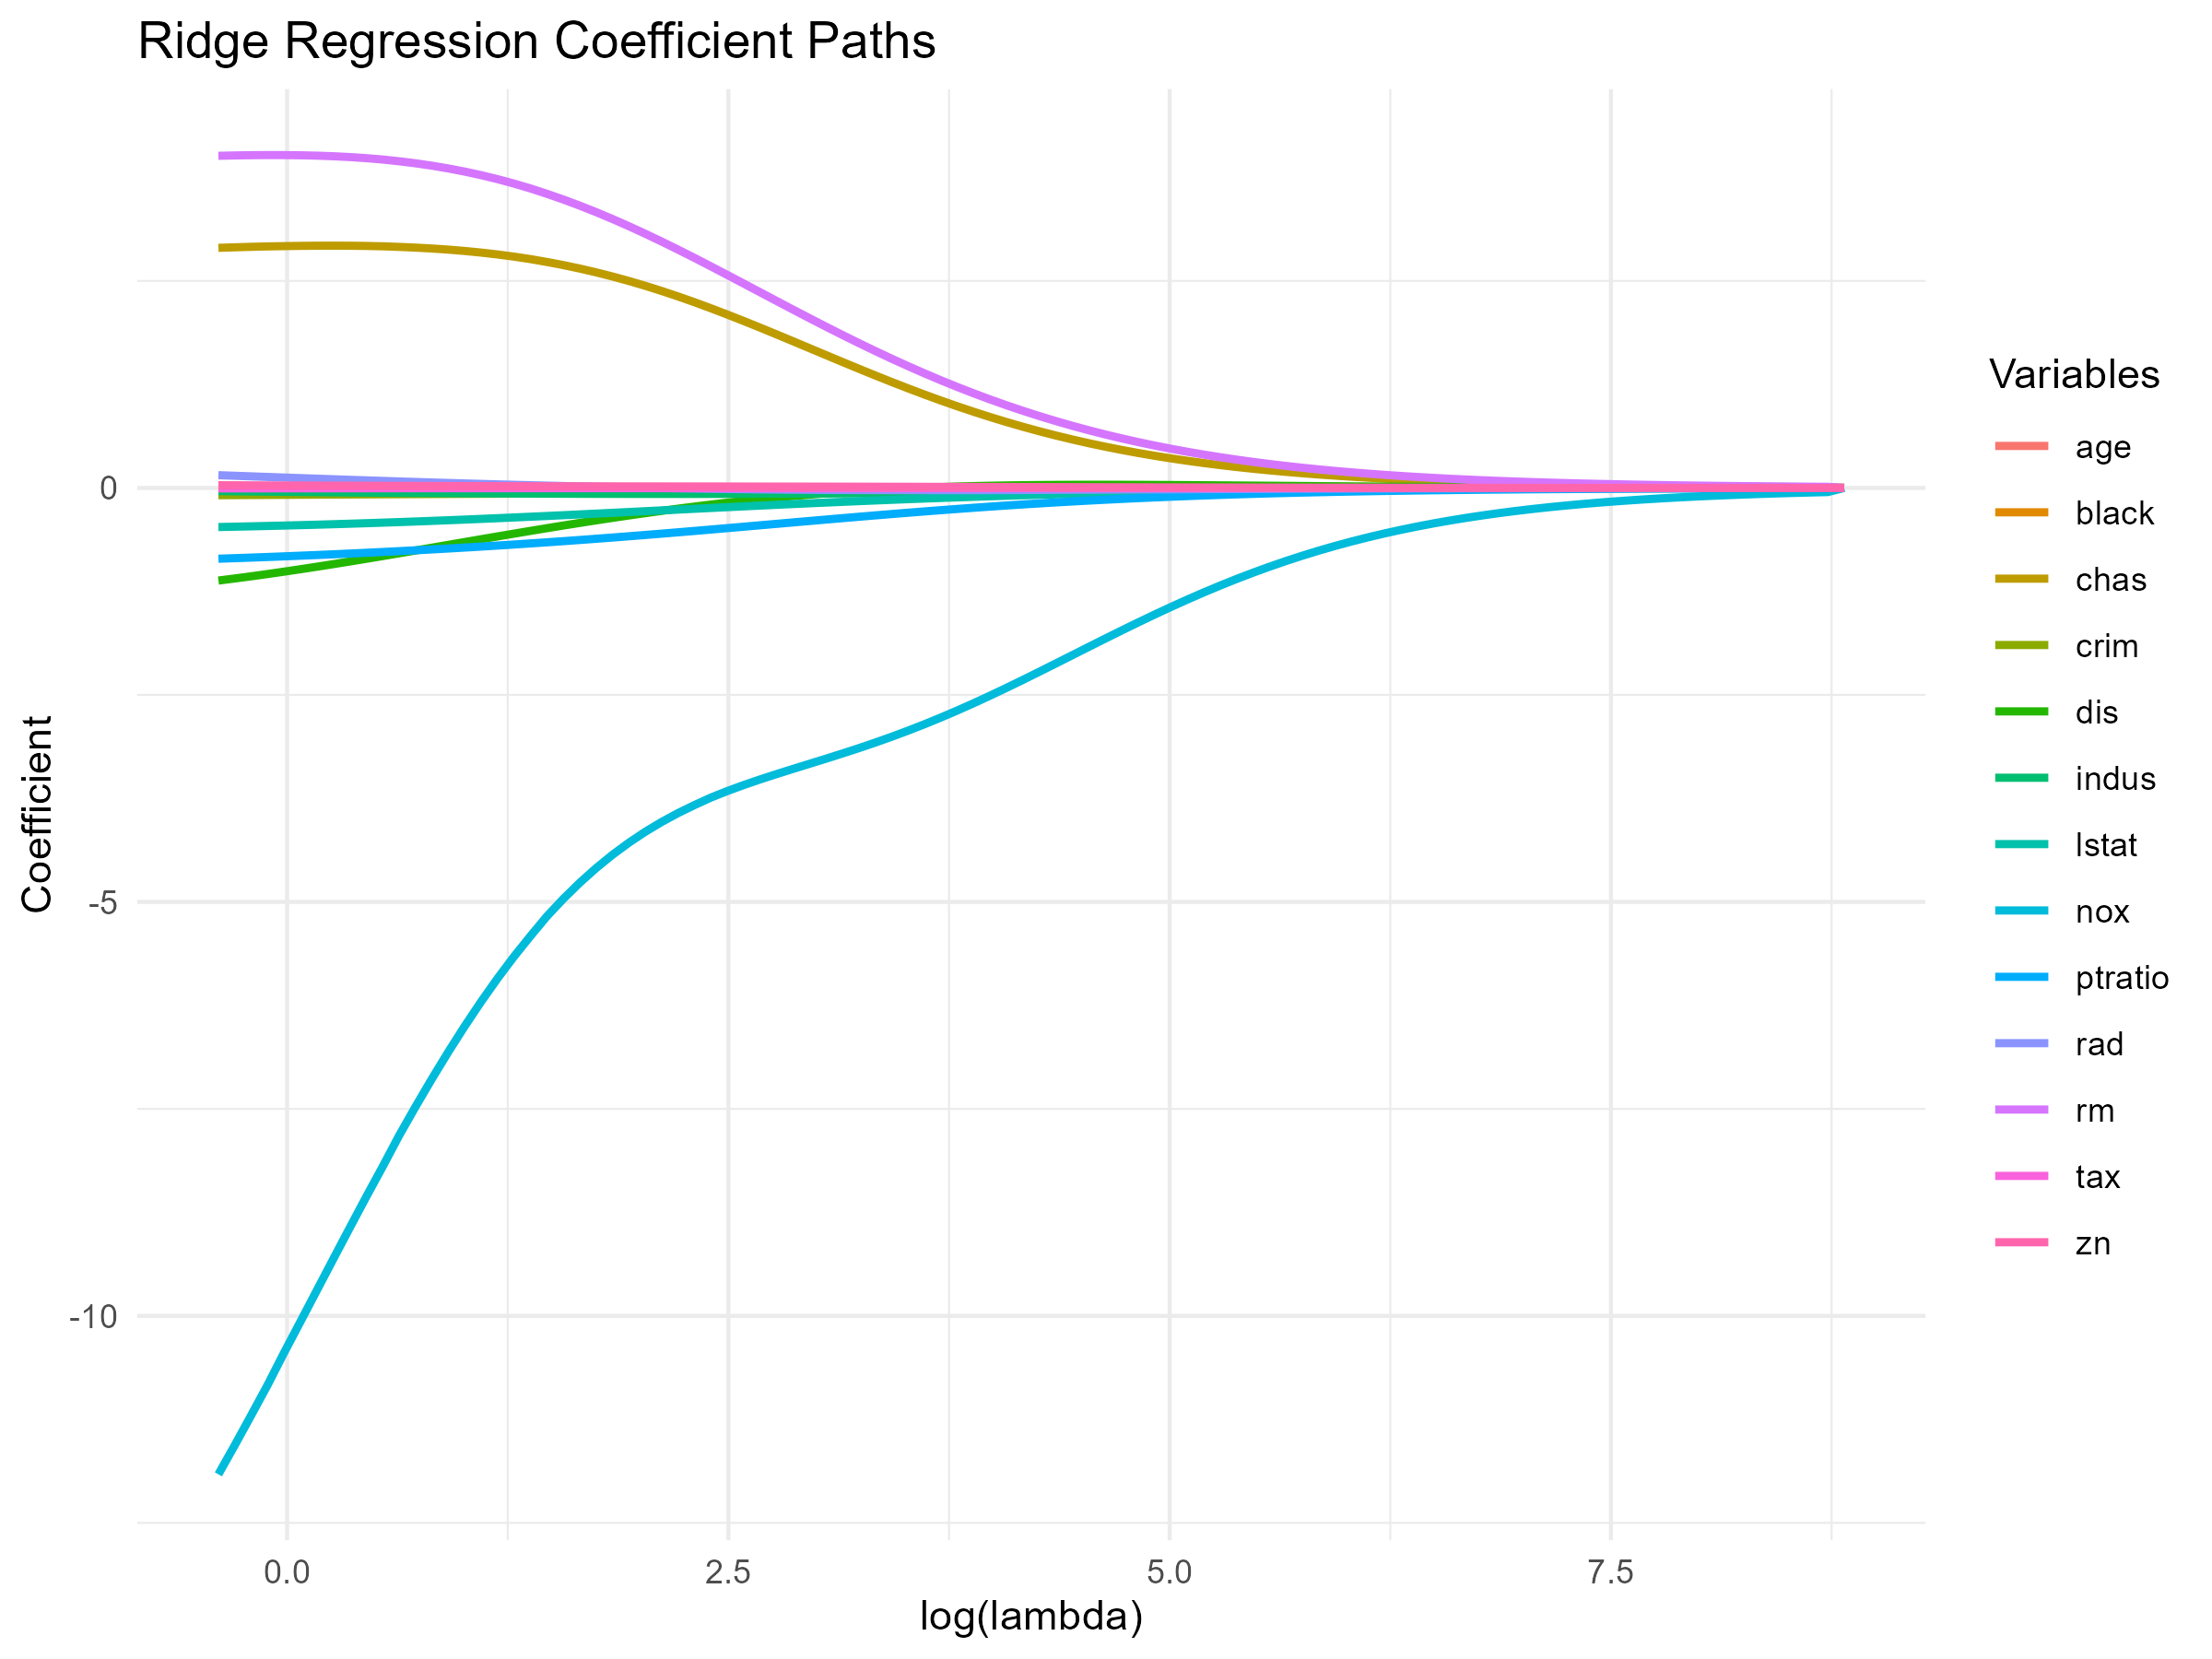
\includegraphics[width=0.75\columnwidth]{../Figure/ridge_coefficients_loglambda.png}
		\caption{岭回归估计随着$\lambda$变化的路径图.}
		\label{fig:ridge_coefficients_loglambda}
	\end{figure}
	\begin{lstlisting}[language=R]
		ridge_plot <- ggplot(ridge_tidy, aes(x = log_lambda, y = estimate, color = term)) +
		geom_line(linewidth = 1) +
		labs(
		title = "Ridge Regression Coefficient Paths",
		x = "log(lambda)", y = "Coefficient"
		) +
		theme_minimal() +
		theme(legend.position = "right") +
		guides(color = guide_legend(title = "Variables"))
	\end{lstlisting}
	
	从图\eqref{fig:ridge_coefficients_loglambda}中可以看出,随着调节参数$\lambda$的增大,岭回归估计向原点收缩,但并不会使任何回归系数严格等于零.				
	
	\begin{figure}[H]
		\small
		\centering
		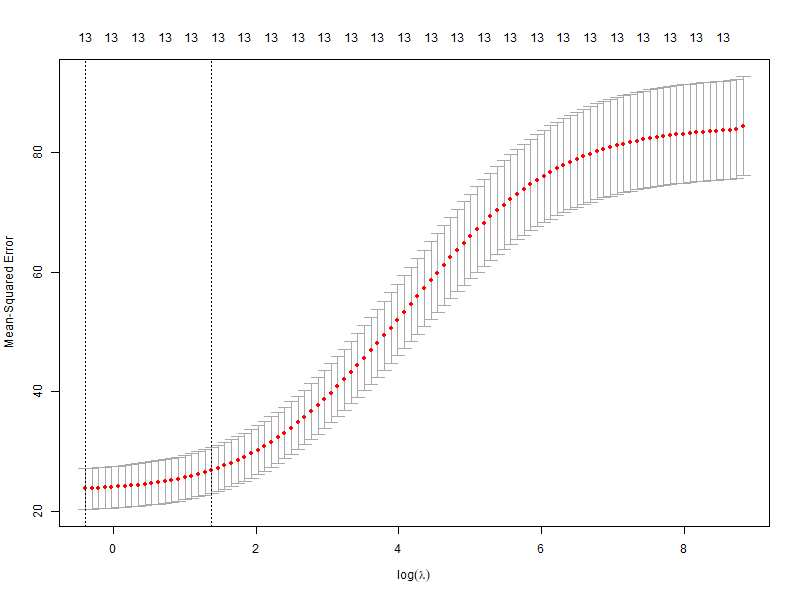
\includegraphics[width=0.8\columnwidth]{../Figure/ridge_cv_plot.png}
		\caption{岭回归的交叉验证误差图.}
		\label{fig:ridge_cv_plot}
	\end{figure}
	使用程序包\texttt{glmnet}中的函数\texttt{cv.glmnet()}选择最优的$\lambda$,并绘制交叉验证误差图,见图\eqref{fig:ridge_cv_plot}.
	
	\begin{lstlisting}[language=R]
		set.seed(2025)
		cv.ridge <- cv.glmnet(x, y, alpha = 0)
		plot(cv.ridge, xlab = expression(log(lambda)))
	\end{lstlisting}
	
	对于图\eqref{fig:ridge_cv_plot},横轴为$\log(\lambda)$,而纵轴为交叉验证误差,同时图上还显示了交叉验证误差的正、负标准差. 左边的垂直虚线表示能使得交叉验证误差最小的$\log(\hat{\lambda})$取值. 右边的垂直虚线表示比$\hat{\lambda}$更大,且与CV($\hat{\lambda}$)相距一个标准差的调节参数的取值,记为$\log(\tilde{\lambda})$. 用\texttt{cv.ridge\$lambda.min}获得$\hat{\lambda }= 0.6777654$;用\texttt{cv.ridge\$lambda.1se}获得$\tilde{\lambda }= 3.969686$.
	
	我们可以提取岭回归系数,结果见附录.
	\begin{lstlisting}[language=R]
		cv.ridge$lambda.min
		cv.ridge$lambda.1se
		coef(cv.ridge, s = "lambda.min")
		coef(cv.ridge, s = "lambda.1se")
	\end{lstlisting}
	
	\subsection{Lasso方法}
	\subsubsection{模型原理}
	岭回归的一个劣势是不能产生稀疏模型,即岭回归方法产生的最终模型还是包含 $p$ 个预测变量,惩罚项 $\lambda \sum_{j=1}^{p} \beta_j^2$ 随着 $\lambda$ 的增大可以把回归系数往 $0$ 的方向推进压缩,但不会把任一个变量的回归系数压缩到 $0$(除非 $\lambda = \infty$).
	
	
	
	为了进行变量选择,考虑下面的惩罚最小二乘目标函数:
	
	\begin{equation}
		Q(\bm{\beta}) = \frac{1}{2n} \|\bm{Y} - \bm{X}\bm{\beta} \|_2^2 + \sum_{j=1}^{p} p_{\lambda}(|\beta_j|)
	\end{equation}
	
	其中 $p_{\lambda}(\cdot)$ 是惩罚函数,$\lambda$ 是调节参数或截断参数,是用来控制模型的复杂度,可以采用交叉验证(CV)方法、广义交叉验证(GCV)方法或 BIC 等数据驱动的准则进行选取. 一个好的惩罚函数应具有无偏性、稀疏性和连续性的性质.
	
	Tibshirani把$L_{1}$惩罚函数施加于回归模型的一般最小二乘和似然函数,提出了Lasso变量选择方法.
	
	针对多元线性回归模型\eqref{lm},极小化下面的 $L_1$ 惩罚最小二乘目标函数,可得回归系数 $\bm{\beta}$ 的 Lasso 估计 $\bm{\hat{\beta}}^L$:
	
	\begin{equation}
		\frac{1}{2n} \sum_{i=1}^{n} \left( y_i - \sum_{j=1}^{p} \beta_j x_{ij} \right)^2 + \lambda \sum_{j=1}^{p} |\beta_j|. \label{lasso}
	\end{equation}
	
	Lasso 估计 $\bm{\hat{\beta}}^L$ 也等价于求解下面的约束优化问题:
	
	\begin{equation}
		\left\{
		\begin{aligned}
			&\min_{\bm{\beta}} \quad \frac{1}{2n} \sum_{i=1}^{n} \left( y_i - \sum_{j=1}^{p} \beta_j x_{ij} \right)^2, \\
			&\text{s.t.} \quad \sum_{j=1}^{p} |\beta_j| \leq c,
		\end{aligned}
		\right. \label{equivLasso}
	\end{equation}
	
	其中非负参数 $c$ 的作用相同于调节参数 $\lambda$,$c$ 的大小控制着 $\sum_{j=1}^{p} |\beta_j|$ 的大小. 随着 $c$ 的变小,约束条件 $\sum_{j=1}^{p} |\beta_j| \leq c$ 的作用会变强,这时会把回归系数接近于 0 的参数压缩到 0,从而产生稀疏模型. 寻找 Lasso 估计,就是寻找最优的调节参数 $\lambda$ 或控制最大 $L_1$ 范数的 $c$,找使得 RSS 最小的回归系数估计.而对于调节参数 $\lambda$,可以通过一些数据驱动的方法进行选取,如 CV、GCV 或 BIC 准则进行选取.
	
	岭回归只能满足连续性,而Lasso方法能够满足稀疏性和连续性.
	
	Hastie 和 Tibshirani (1990) 定义了有效的自由度,它表示模型的复杂度. 为了定义 Lasso 的自由度,首先给出下面的 Stein 引理.
	\begin{lemma}
		假设 $\hat{\bm{\mu}}: \mathbb{R}^n \to \mathbb{R}^n$ 是几乎处处可微的,且令
		\[
		\nabla \cdot\hat{\bm{\mu}} = \sum_{i=1}^{n} \frac{\partial \hat{\mu}_i}{\partial y_i}.
		\]
		如果 $\bm{Y} \sim N_n(\bm{\mu}, \sigma^2 \bm{I}_n)$,则有
		\[
		\sum_{i=1}^{n} \operatorname{Cov}(\hat{\mu}_i, y_i)/\sigma^2 = \mathbb{E}[\nabla \cdot \hat{\bm{\mu}}].
		\]\label{lem:Stein}
	\end{lemma} 
	
	假设一个同方差模型:$\bm{Y} \sim N(\bm{\mu}, \sigma^2 \bm{I}_n)$. 对任何估计:$\hat{\bm{\mu}} = \delta(\bm{Y})$,引理\eqref{lem:Stein} 定义了 $\hat{\bm{\mu}}$ 的自由度:
	
	\begin{equation}
		df(\hat{\bm{\mu}}) = \sum_{i=1}^{n} \operatorname{Cov}(\hat{\mu}_i, y_i)/\sigma^2.
	\end{equation}
	
	自由度表示模型的复杂度,即回归系数估计的非零系数的个数. 对给定的调节参数 $\lambda$,令 $\hat{\bm{\beta}}(\lambda)$ 表示回归系数向量 $\bm{\beta}$ 的 Lasso 估计,则 Lasso 的自由度定义为:
	\begin{equation}
		df(\lambda) = \#\{j : \hat{\beta}_j(\lambda) \neq 0\},
	\end{equation}

	其中 $\#$ 表示集合中元素的个数. 可知$df(\lambda) = \mathbb{E}[\widehat{df}(\lambda)]$,则 $df(\lambda)$ 是 Lasso 自由度的无偏估计.
	
	有了自由度的定义,在实际应用中,可以使用 GCV 方法和 BIC 方法选取调节参数 $\lambda$.
	
	\textbf{GCV 方法} \quad 可以极小化下面的 GCV 准则选择调节参数 $\lambda$,即
	\[
	\hat{\lambda}_{\text{gcv}} = \arg\min_{\lambda} \text{GCV}(\lambda) = \arg\min_{\lambda} \frac{\|\bm{Y} - \bm{X}\hat{\bm{\beta}}_{\lambda}\|_2^2}{n(1 - \hat{df}(\lambda)/n)^2},
	\]
	其中 $\hat{\bm{\beta}}_{\lambda}$ 表示给定 $\lambda$ 时极小化 $L_1$ 惩罚最小二乘目标函数 \eqref{lasso}的 Lasso 估计,且 $\hat{df}(\lambda)$ 表示给定 $\lambda$ 的自由度.
	
	\textbf{BIC 方法} \quad 可以通过极小化下面的 BIC 准则进行选择调节参数 $\lambda$,即
	\[
	\text{BIC}(\lambda) = \log \hat{\sigma}^2_{\lambda} + \frac{\hat{df}(\lambda) \log(n)}{n},
	\]
	其中 $\hat{\sigma}^2_{\lambda}$ 是基于任一 $\lambda$ 所得模型的残差平方和除以 $n$.极小化上面的 BIC 准则目标函数 $\text{BIC}(\lambda)$,可以选择最优的调节参数 $\lambda$,记为 $\hat{\lambda}_{\text{bic}}$.
	
	\subsubsection{代码实践}
	\begin{example}
		用程序包\texttt{glmnet}中的函数\texttt{glmnet()}对波士顿房价数据进行Lasso回归分析.
	\end{example}
	
	Lasso回归只需将岭回归中\texttt{glmnet()}函数参数\texttt{alpha}设置为1.
	
	\begin{lstlisting}[language=R]
		fit_lasso <- glmnet(x, y, alpha = 1, nlambda = 100)
		lasso_tidy <- tidy(fit_lasso) %>%
		filter(term != "(Intercept)") %>%
		mutate(log_lambda = log(lambda))
		lasso_plot <- ggplot(lasso_tidy, aes(x = log_lambda, y = estimate, color = term)) +
		geom_line(linewidth = 1) +
		labs(
		title = "lasso Regression Coefficient Paths",
		x = "log(lambda)", y = "Coefficient"
		) +
		theme_minimal() +
		theme(legend.position = "right") +
		guides(color = guide_legend(title = "Variables"))
	\end{lstlisting}
	
	\begin{figure}[H]
		\small
		\centering
		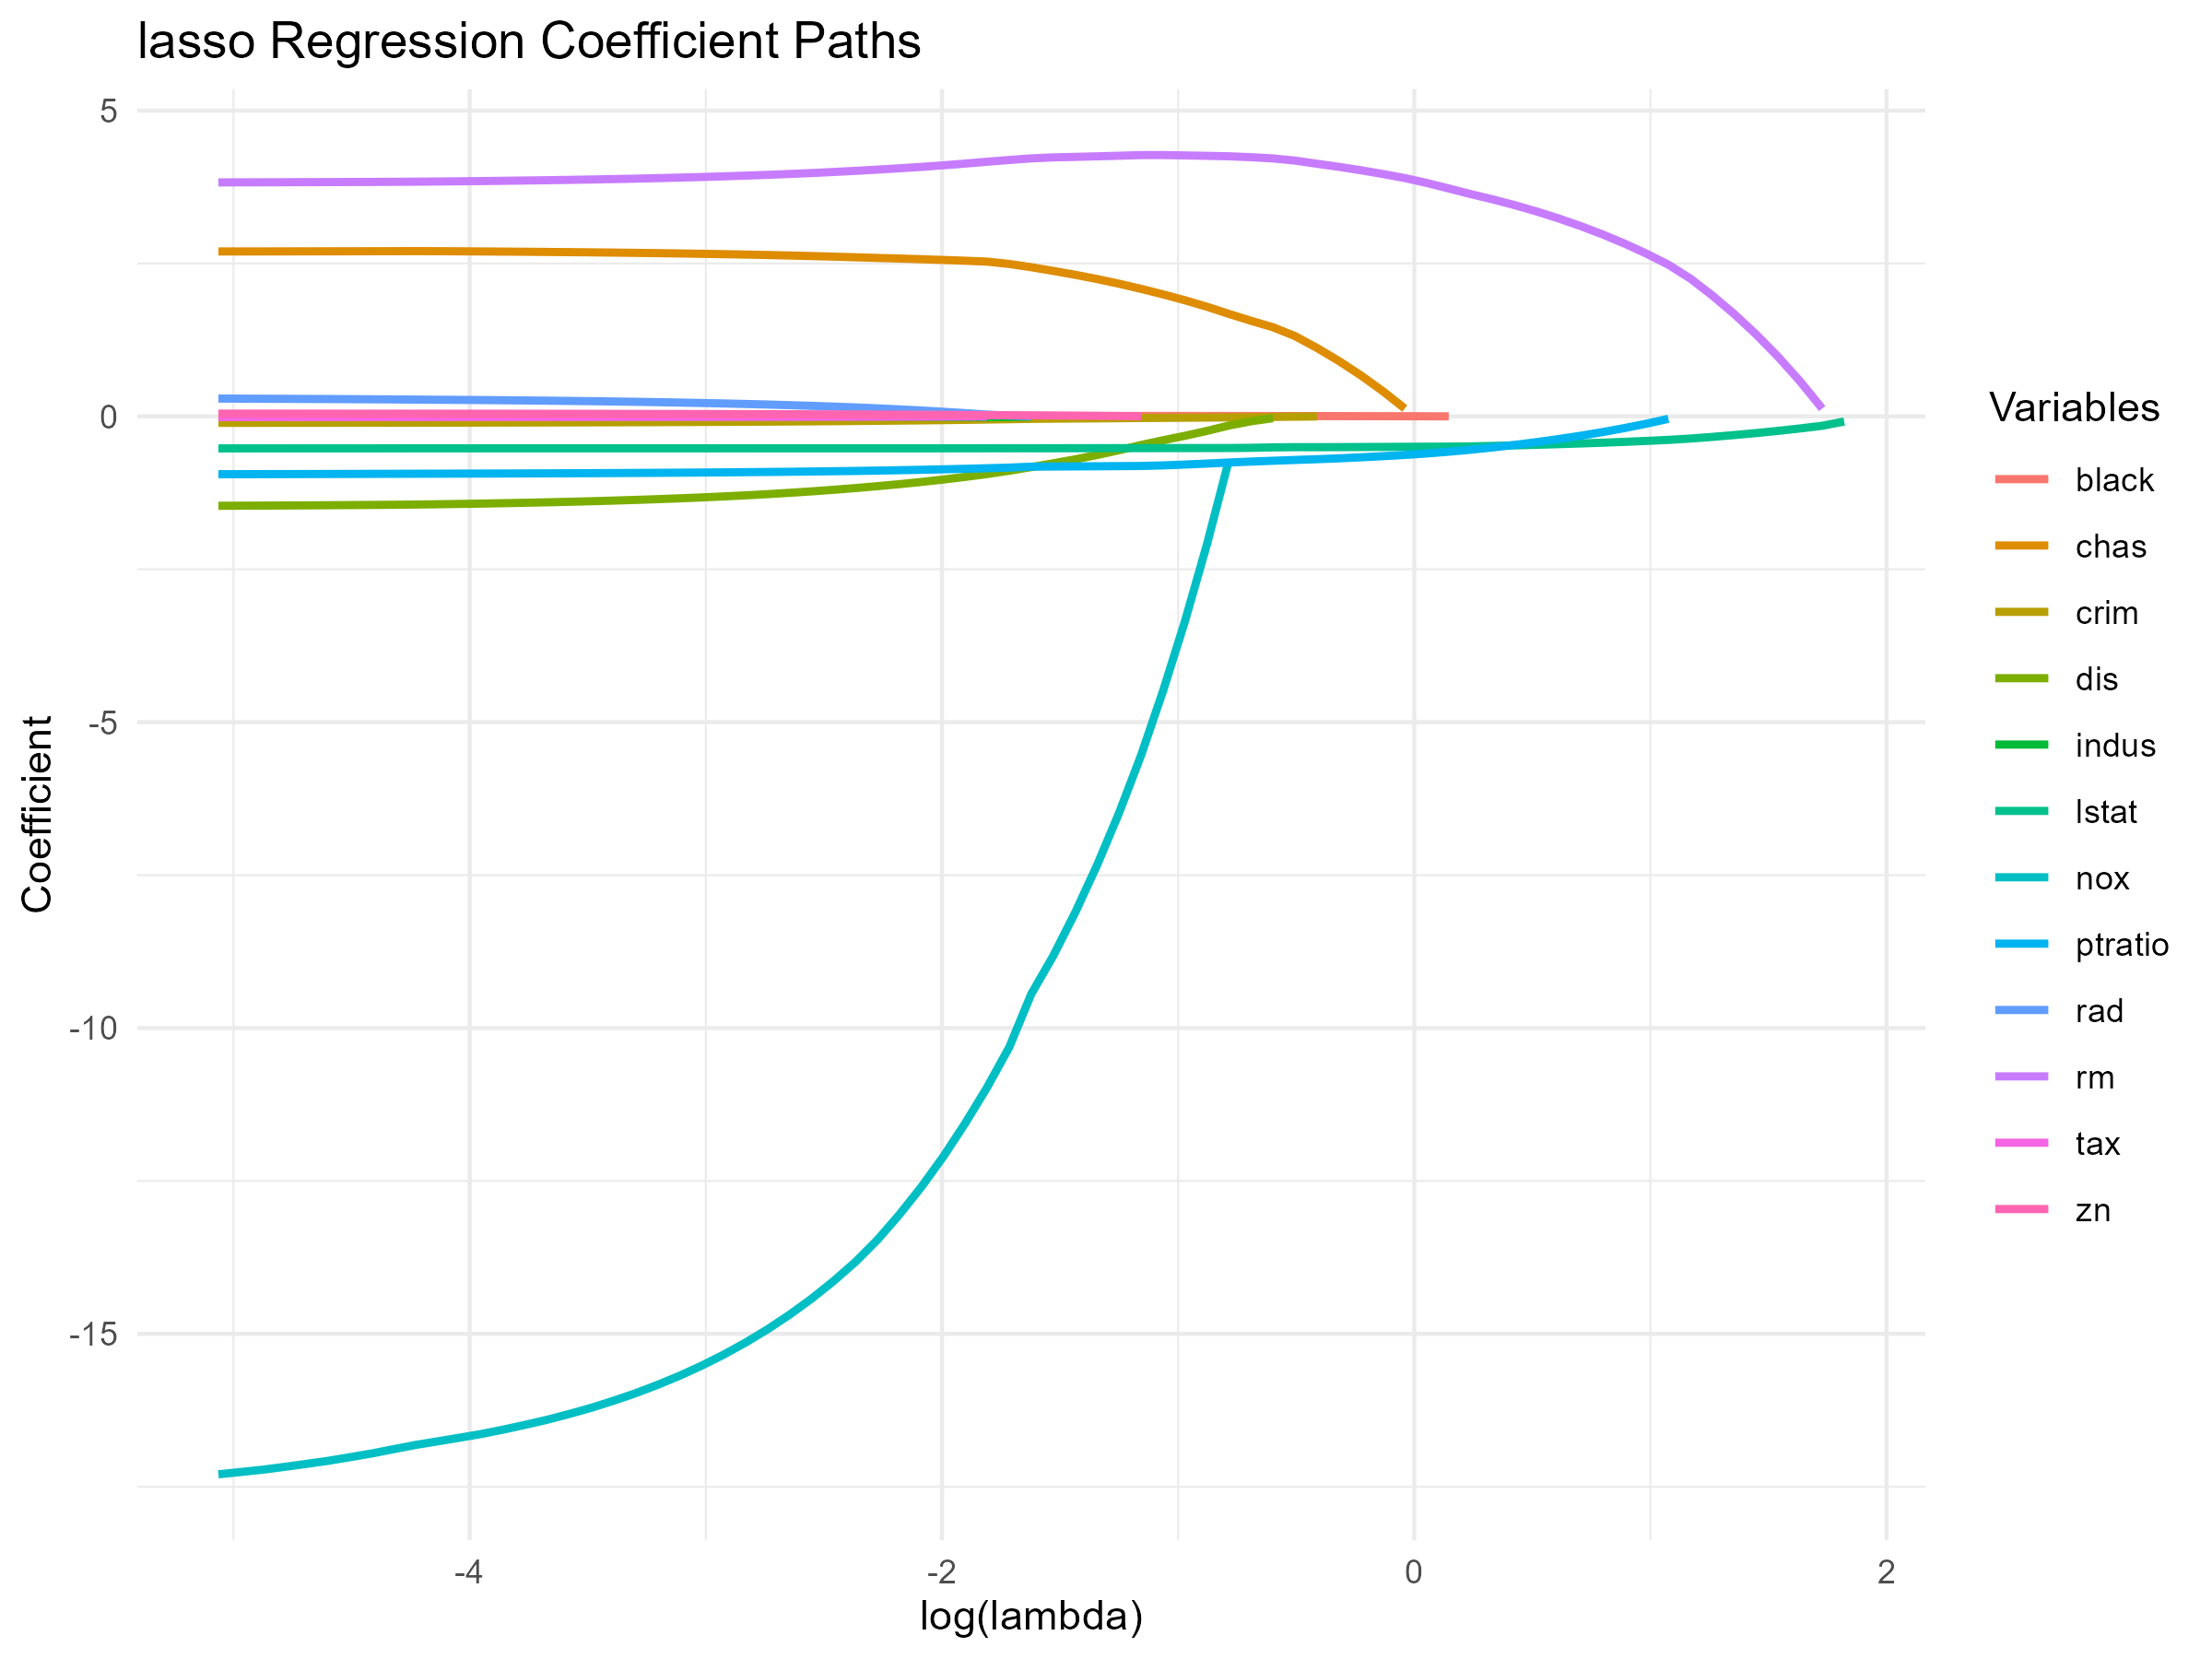
\includegraphics[width=0.8\columnwidth]{../Figure/lasso_coefficients_loglambda.png}
		\caption{Lasso回归估计随着$\lambda$变化的路径图.}
		\label{fig:lasso_coefficients_loglambda}
	\end{figure}
	
	从图\eqref{fig:lasso_coefficients_loglambda}中可以看出,$\lambda$足够大时,Lasso回归估计得到一个零模型,所有回归系数的Lasso估计均为$0$. 因此,根据不同$\lambda$的取值,可以得到包含不同变量的模型,说明了Lasso方法筛选变量的功能.			
	
	同样,我们可以绘制交叉验证误差图,见图\eqref{fig:lasso_cv_plot}.
	\begin{lstlisting}[language=R]
		set.seed(2025)
		cv.lasso <- cv.glmnet(x, y, alpha = 1)
		plot(cv.lasso, xlab = expression(log(lambda)))
	\end{lstlisting}
	\begin{figure}[H]
		\small
		\centering
		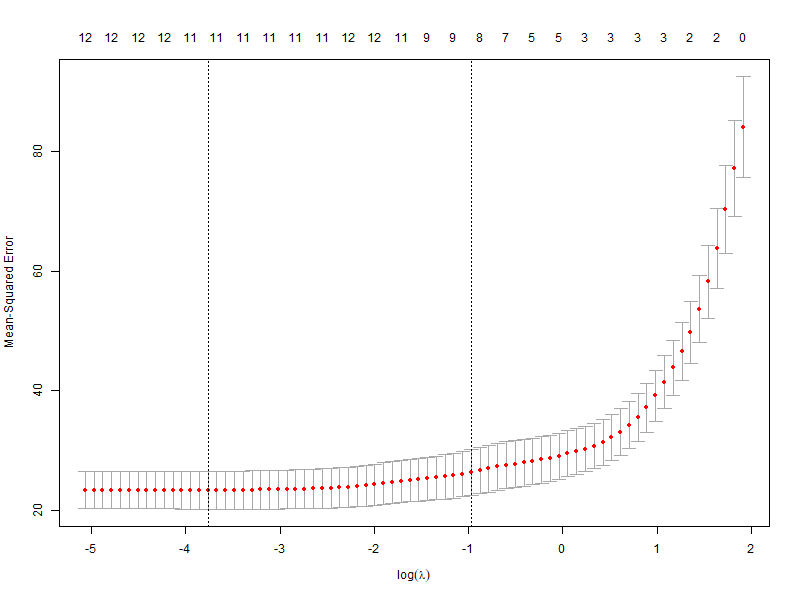
\includegraphics[width=0.8\columnwidth]{../Figure/lasso_cv_plot.png}
		\caption{Lasso回归的交叉验证误差图.}
		\label{fig:lasso_cv_plot}
	\end{figure}
	从\eqref{fig:lasso_cv_plot}中可见使得CV($\hat{\lambda}$)最小化的$\lambda$为$\hat{\lambda} = 0.02325053$, 而利用“一个标准差”准则选取的$\lambda$为$\tilde{\lambda} = 0.3789258$. 我们可以用函数\texttt{coef()}分别提取$\hat{\lambda}$和$\tilde{\lambda}$对应的回归系数的Lasso估计.
	\begin{lstlisting}[language=R]
		cv.lasso$lambda.min
		cv.lasso$lambda.1se
		coef(cv.lasso, s = "lambda.min")
		coef(cv.lasso, s = "lambda.1se")
	\end{lstlisting}
	从结果看来,部分回归系数为0,即得到了稀疏解,使得模型更为简单,不易导致过拟合.
	
	\subsection{SCAD回归}
	\subsubsection{模型建立}
	先前提到的惩罚函数不能同时满足无偏性、稀疏性和连续性。为了解决这个问题,Fan (1997) 提出了一个连续可微的惩罚函数,称为 SCAD 惩罚函数:
	\begin{equation}
		p_{\lambda}'(|\theta|) = \lambda \left\{ I(|\theta| \leq \lambda) + \frac{(a\lambda - |\theta|)_{+}}{(a - 1)\lambda} I(|\theta| > \lambda) \right\}, \label{SCADFun}
	\end{equation}
	
	针对多元线性模型\eqref{lm},考虑下面的 SCAD 惩罚最小二乘目标函数:
	\begin{equation}
		Q(\bm{\beta}) = \frac{1}{2n} \|\bm{Y} - \bm{X}\bm{\beta} \|_2^2 + \sum_{j=1}^{p} p_{\lambda}(|\beta_j|), \label{SCAD}
	\end{equation}
	其中 $p_{\lambda}(\cdot)$ 是由式\eqref{SCADFun}定义的 SCAD 惩罚函数,$\lambda$ 是调节参数或截断参数. 极小化$Q(\bm{\beta})$可得回归系数向量的一个SCAD估计$\hat{\bm{\beta}}$. 为求解,可利用LQA算法.
	
	\subsubsection{代码实践}
	\begin{example}
		用程序包\texttt{neverge}中的函数\texttt{nevreg()}对波士顿房价数据进行SCAD回归分析.
	\end{example}
	
	进行SCAD回归.
	\begin{lstlisting}[language=R]
		library(MASS)
		library(ncvreg)
		library(ggplot2)
		library(reshape2)
		data("Boston")
		x <- as.matrix(Boston[, -14])
		y <- Boston$medv
		fit_SCAD <- ncvreg(x, y, family = "gaussian", penalty = "SCAD", nlambda = 100)
	\end{lstlisting}
	
	可以绘制SCAD估计随着$\lambda$变化的路径图以及交叉验证误差图.
	\begin{figure}[H]
		\small
		\centering
		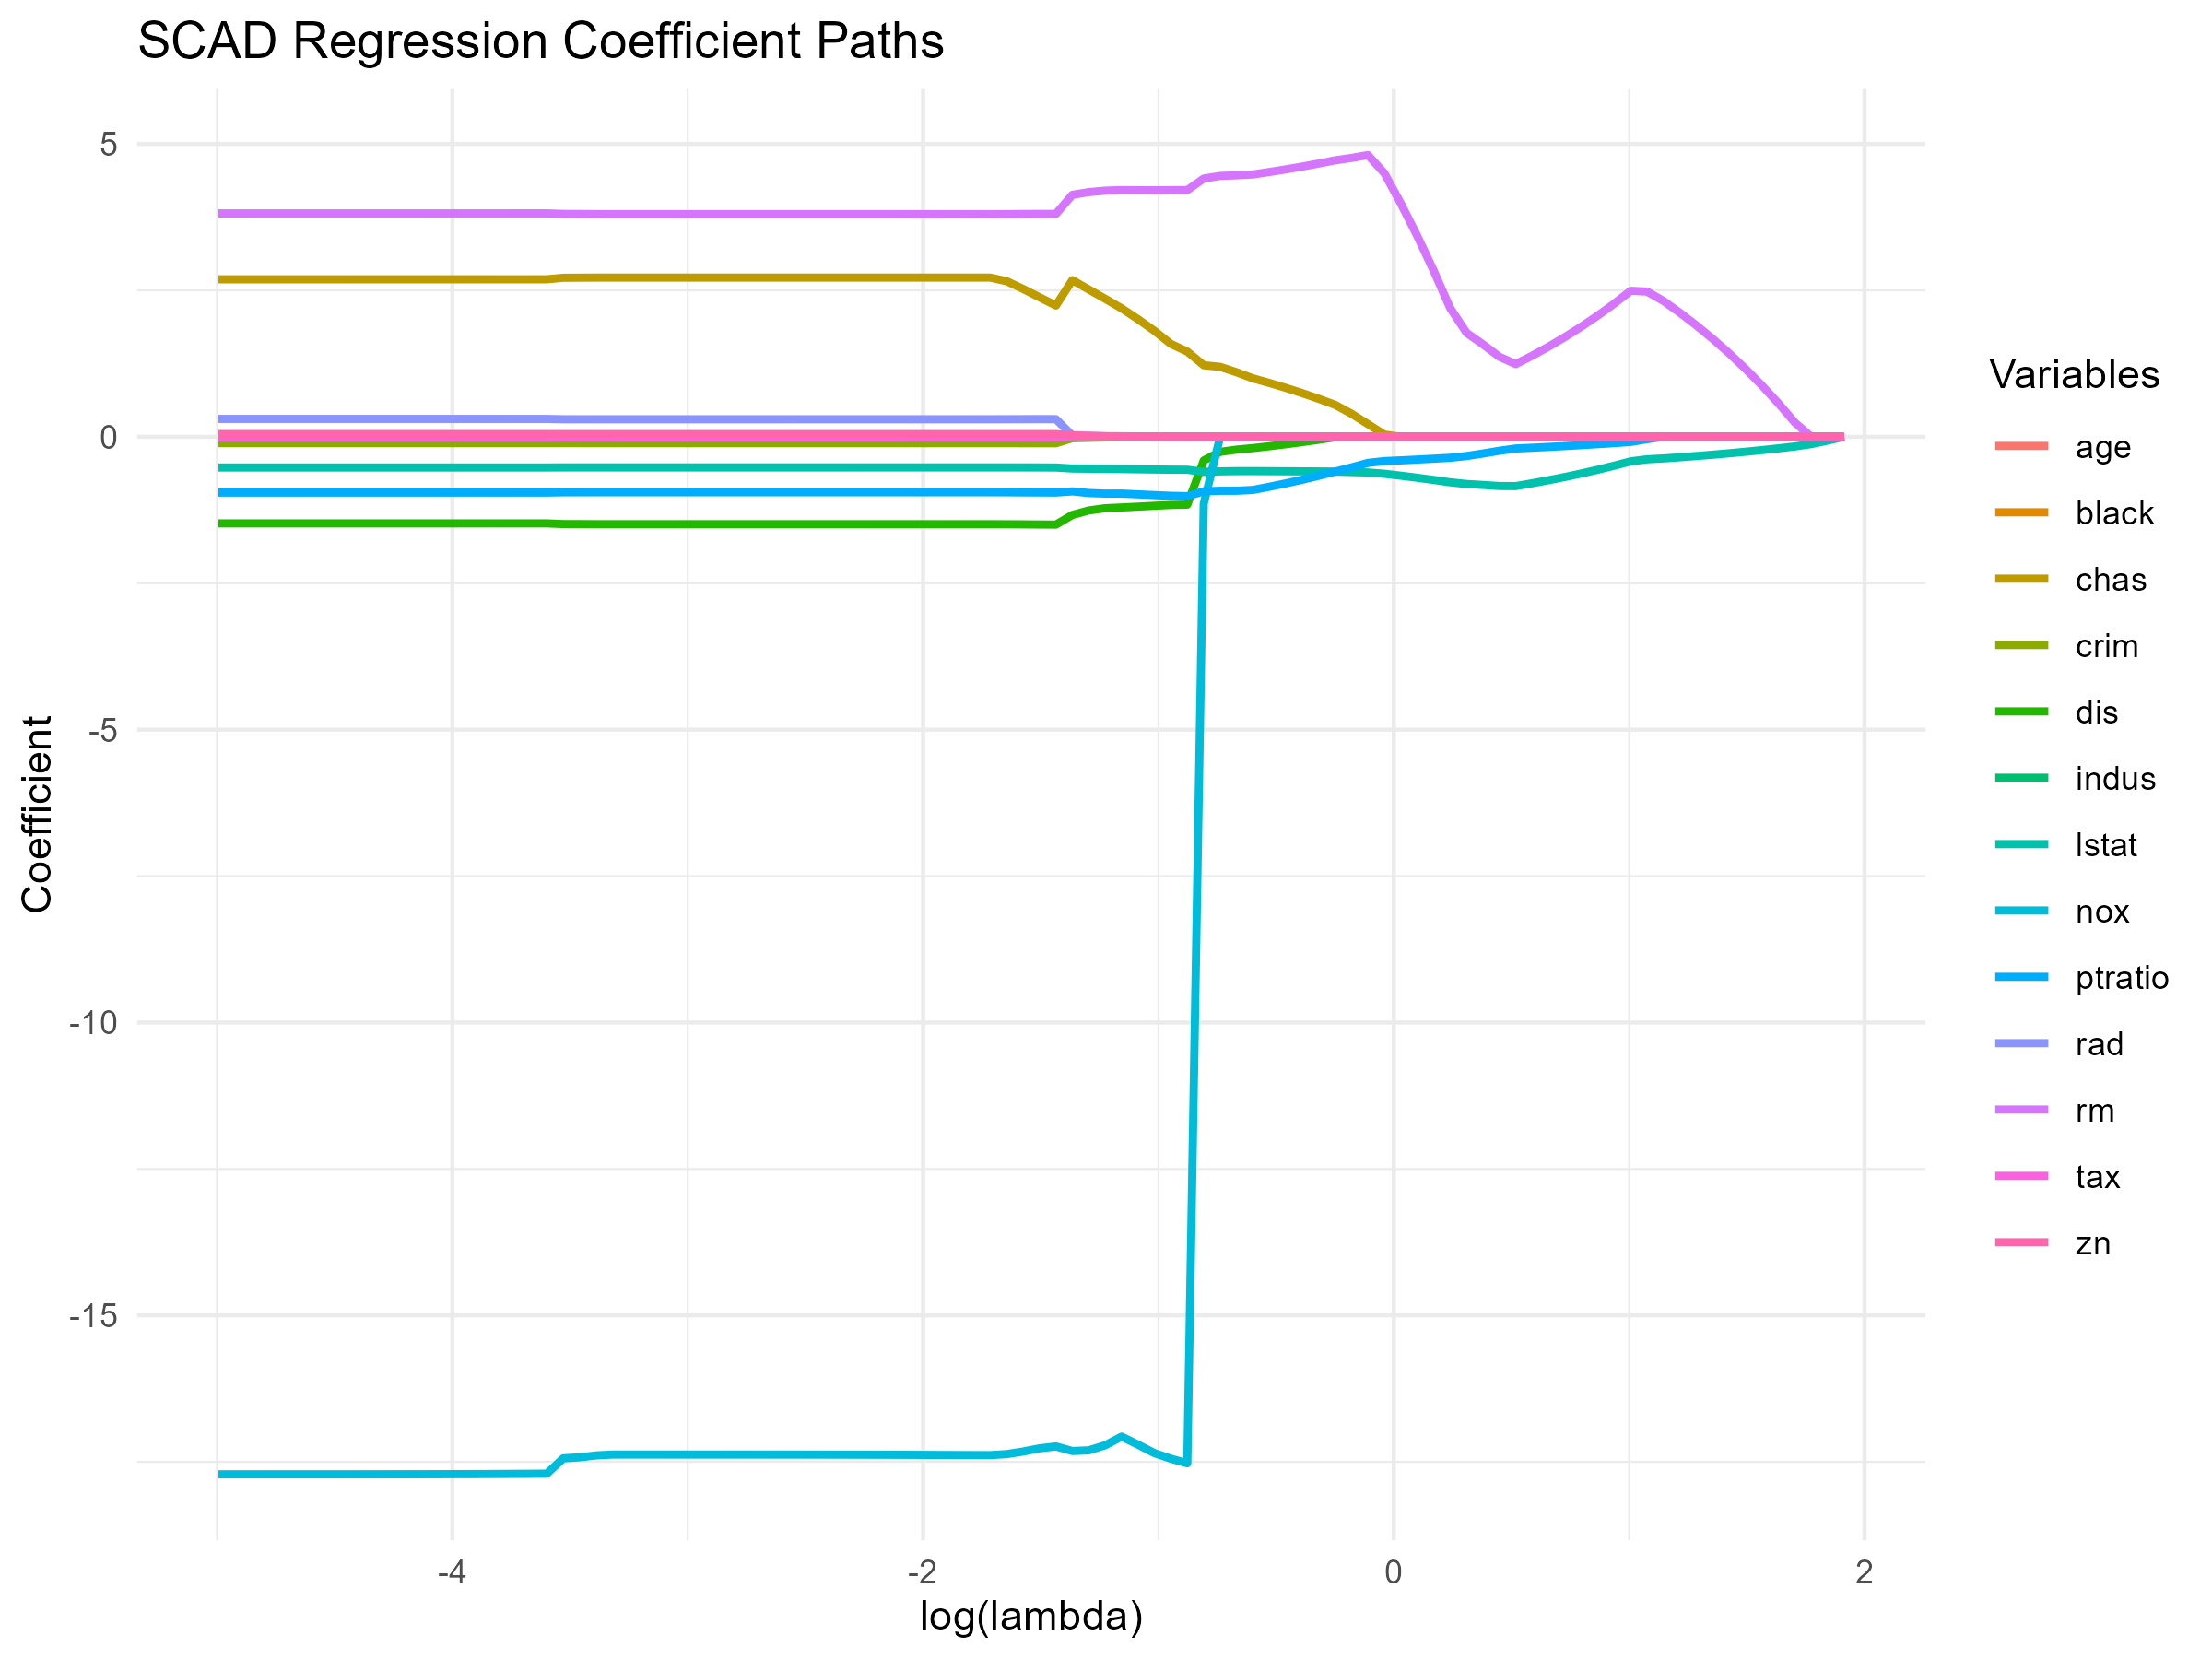
\includegraphics[width=0.75\columnwidth]{../Figure/SCAD_coefficients_loglambda.png}
		\caption{SCAD回归估计随着$\lambda$变化的路径图.}
		\label{fig:SCAD_coefficients_loglambda}
	\end{figure}
	图\eqref{fig:SCAD_coefficients_loglambda}显示了SCAD估计的路径图.类似于Lasso方法,随着$\lambda$的取值变化,可以得到包含不同变量的模型,具有筛选变量的作用.
	\begin{figure}[H]
		\small
		\centering
		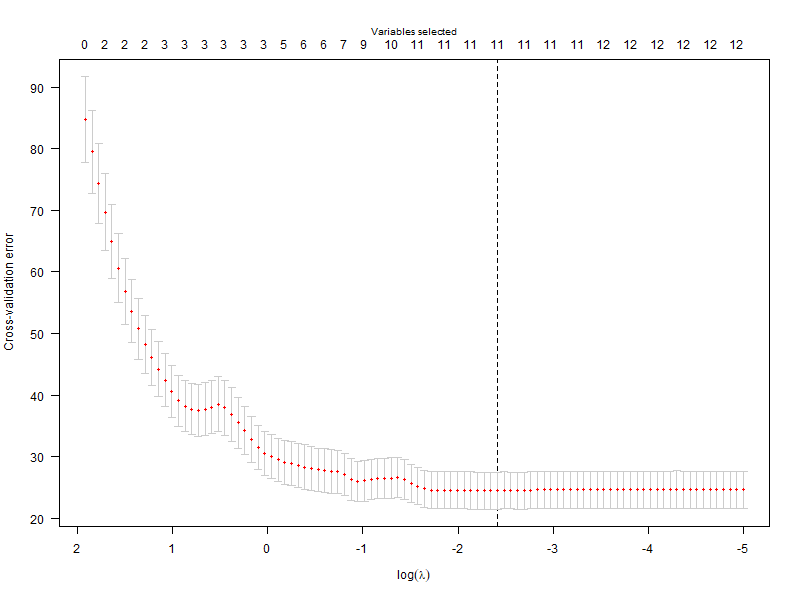
\includegraphics[width=0.75\columnwidth]{../Figure/SCAD_cv_plot.png}
		\caption{SCAD回归的交叉验证误差图.}
		\label{fig:SCAD_cv_plot}
	\end{figure}
	图\eqref{fig:SCAD_cv_plot}展示了交叉验证误差图.
	
	\subsection{自适应Lasso}
	\subsubsection{模型构建}
	我们先前得到了 Lasso 估计:
	\begin{equation}
		\hat{\bm{\beta}}^L = \arg\min_{\bm{\beta}} \left\{ \frac{1}{2n} \|\bm{Y} - \bm{X}\bm{\beta} \|_2^2 + \lambda \|\bm{\beta} \|_1 \right\},
	\end{equation}
	
	其中 $\|\bm{\beta} \|_1 = \sum_{j=1}^{p} |\beta_j|$。令 $\mathcal{A} = \{j : \beta_{0j} \ne 0\}$ 表示活动模型,$\hat{\mathcal{A}}_n = \{j : \hat{\beta}_j^L \ne 0\}$ 表示选择模型。变量选择的目的就是希望能正确识别正确的模型,即理论上需要证明下面变量选择相合性,即
	\[
	\lim_{n \to \infty} \Pr(\hat{A}_n = A) = 1.
	\]
	而Lasso估计不满足,因此引出自适应Lasso估计.
	令 $\hat{\bm{\beta}}$ 是 $\bm{\beta}$ 的一个 $\sqrt{n}$-相合估计,如最小二乘估计. 定义权向量:$\hat{\bm{w}} = 1 / |\hat{\bm{\beta}}|^{\gamma}$,$\gamma > 0$。自适应 Lasso 估计 $\hat{\bm{\beta}}^{\text{alasso}}$ 定义为:
	
	\begin{equation}
		\hat{\bm{\beta}}^{\text{alasso}} = \arg \min_{\bm{\beta}} \left\{ \frac{1}{2n} \|\bm{Y} - \bm{X}\bm{\beta}\|_2^2 + \lambda \sum_{j=1}^{p} \hat{w}_j |\beta_j| \right\}. \label{alasso}
	\end{equation}
	
	从自适应 Lasso 估计式 \eqref{alasso} 可知,自适应 Lasso 的基本思想是,对于最小二乘估计大的回归系数,不进行惩罚,而对于接近于 0 的回归系数给予尽量大的惩罚,并压缩到 0. 如果选取合适的 $\gamma$,自适应 Lasso 的解将满足无偏性、稀疏性和连续性. 求解自适应Lasso可以利用LARS算法.
	
	\subsubsection{代码实践}
	\begin{example}
		用程序包\texttt{msgps()}对波士顿房价数据进行自适应Lasso回归分析.
	\end{example}
	
	可以直接通过\text{msgps()}进行自适应Lasso分析:
	\begin{lstlisting}[language=R]
		library(msgps)
		library(MASS)
		
		# 加载 Boston 数据
		data("Boston")
		x <- as.matrix(Boston[, -14])
		y <- Boston$medv
		
		# 自适应Lasso回归
		alasso_fit <- msgps(x, y, penalty = "alasso", gamma = 1, lambda = 0)
		
		# 绘图
		png("alasso_plot.png", width = 800, height = 400)
		par(mfrow = c(1, 2))
		plot(alasso_fit, criterion = "gcv", xvar = "t", main = "GCV")
		plot(alasso_fit, criterion = "bic", xvar = "t", main = "BIC")
		dev.off()
	\end{lstlisting}
	图\eqref{fig:alasso_plot}展示了分别采用GCV准则和BIC准则选取的调节参数.
	\begin{figure}[H]
		\small
		\centering
		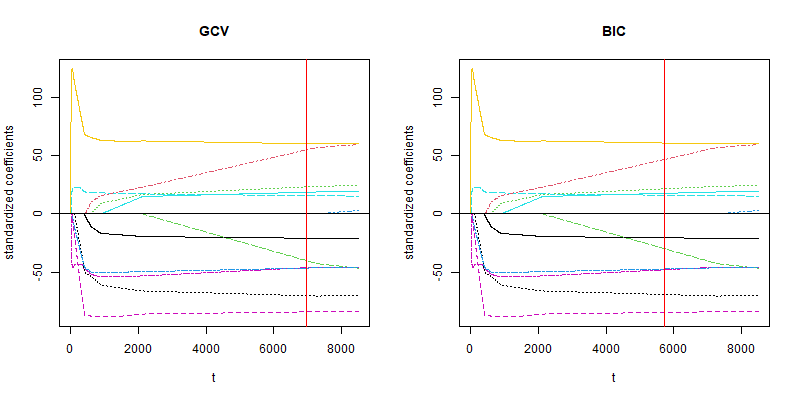
\includegraphics[width=0.8\columnwidth]{../Figure/alasso_plot.png}
		\caption{SCAD回归估计随着$\lambda$变化的路径图.}
		\label{fig:alasso_plot}
	\end{figure}
	
	使用\texttt{summary()}可以对输出结果进行汇总,结果见附录.
	\newpage
	
	\begin{thebibliography}{99}
		\bibitem{a}李高荣,吴密霞 编著. \emph{多元统计分析}[M]. 北京: 科学出版社, 2021.
	\end{thebibliography}
	
	\newpage
	
	\begin{appendices}
		\renewcommand{\thesection}{\Alph{section}}
		\section{回归系数表}
		\begin{table}[htbp]
			\centering
			\caption{Ridge回归在 $\hat{\lambda}$ 与 $\tilde{\lambda}$ 下的非零系数}
			\vspace{1em}
			
			\begin{minipage}{0.48\textwidth}
				\centering
				\caption*{(a) $\hat{\lambda}$}
				\begin{tabular}{l r l}
					\toprule
					& Coef & Term \\
					\midrule
					(Intercept) & 28.0015 & (Intercept)\\
					crim & -0.0876 & crim\\
					zn & 0.0327 & zn\\
					indus & -0.0380 & indus\\
					chas & 2.8998 & chas\\
					nox & -11.9134 & nox\\
					rm & 4.0113 & rm\\
					age & -0.0037 & age\\
					dis & -1.1189 & dis\\
					rad & 0.1537 & rad\\
					tax & -0.0058 & tax\\
					ptratio & -0.8550 & ptratio\\
					black & 0.0091 & black\\
					lstat & -0.4724 & lstat\\
					\bottomrule
				\end{tabular}
			\end{minipage}
			\hfill
			\begin{minipage}{0.48\textwidth}
				\centering
				\caption*{(b) $\tilde{\lambda}$}
				\begin{tabular}{l r l}
					\toprule
					& Coef & Term \\
					\midrule
					(Intercept) & 20.8162 & (Intercept)\\
					crim & -0.0679 & crim\\
					zn & 0.0204 & zn\\
					indus & -0.0687 & indus\\
					chas & 2.7637 & chas\\
					nox & -5.4131 & nox\\
					rm & 3.6171 & rm\\
					age & -0.0077 & age\\
					dis & -0.5190 & dis\\
					rad & 0.0327 & rad\\
					tax & -0.0029 & tax\\
					ptratio & -0.6703 & ptratio\\
					black & 0.0076 & black\\
					lstat & -0.3479 & lstat\\
					\bottomrule
				\end{tabular}
			\end{minipage}
			
		\end{table}
		
		\begin{table}[htbp]
			\centering
			\caption{Lasso回归在 $\hat{\lambda}$ 与 $\tilde{\lambda}$ 下的非零系数}
			\vspace{1em}
			
			\begin{minipage}{0.48\textwidth}
				\centering
				\caption*{(a) $\hat{\lambda}$}
				\begin{tabular}{l r l}
					\toprule
					& Coef & Term \\
					\midrule
					(Intercept) & 34.7411 & (Intercept)\\
					crim & -0.1000 & crim\\
					zn & 0.0422 & zn\\
					indus & 0.0000 & indus\\
					chas & 2.6914 & chas\\
					\addlinespace
					nox & -16.4841 & nox\\
					rm & 3.8564 & rm\\
					age & 0.0000 & age\\
					dis & -1.4121 & dis\\
					rad & 0.2603 & rad\\
					\addlinespace
					tax & -0.0101 & tax\\
					ptratio & -0.9327 & ptratio\\
					black & 0.0091 & black\\
					lstat & -0.5225 & lstat\\
					\bottomrule
				\end{tabular}
			\end{minipage}
			\hfill
			\begin{minipage}{0.48\textwidth}
				\centering
				\caption*{(b) $\tilde{\lambda}$}
				\begin{tabular}{l r l}
					\toprule
					& Coef & Term \\
					\midrule
					(Intercept) & 17.4715 & (Intercept)\\
					crim & -0.0218 & crim\\
					zn & 0.0000 & zn\\
					indus & 0.0000 & indus\\
					chas & 1.8977 & chas\\
					\addlinespace
					nox & -3.3413 & nox\\
					rm & 4.2663 & rm\\
					age & 0.0000 & age\\
					dis & -0.3171 & dis\\
					rad & 0.0000 & rad\\
					\addlinespace
					tax & 0.0000 & tax\\
					ptratio & -0.7873 & ptratio\\
					black & 0.0066 & black\\
					lstat & -0.5181 & lstat\\
					\bottomrule
				\end{tabular}
			\end{minipage}
			
		\end{table}
		\newpage
		
		\begin{lstlisting}[language=R, caption={自适应Lasso回归的结果}]
			Call: msgps(X = x, y = y, penalty = "alasso", gamma = 1, lambda = 0)
			
			Penalty: "alasso"
			
			gamma: 1
			
			lambda: 0
			
			df:
			tuning      df
			[1,]  0.0000  0.0000
			[2,]  0.3814  0.2484
			[3,]  0.7630  0.4969
			[4,]  1.1444  0.7453
			[5,]  4.0198  1.2183
			[6,]  7.4965  2.1132
			[7,]  9.2763  2.7975
			[8,]  9.4515  3.3418
			[9,] 10.0666  3.7518
			[10,] 10.6814  4.0942
			[11,] 11.2660  4.6070
			[12,] 11.8551  4.9074
			[13,] 12.7180  5.4213
			[14,] 14.0164  6.6353
			[15,] 15.5274  7.6835
			[16,] 16.6140  8.7381
			[17,] 17.2934  9.7463
			[18,] 17.7604 10.2261
			[19,] 18.2293 10.6565
			[20,] 23.6064 12.7498
			
			tuning.max: 23.61
			
			ms.coef:
			Cp       AICC        GCV        BIC
			(Intercept)  36.286119  36.286119  36.286119  36.195154
			crim         -0.107663  -0.107663  -0.107663  -0.105748
			zn            0.044418   0.044418   0.044418   0.041215
			indus         0.000000   0.000000   0.000000   0.000000
			chas          2.750745   2.750745   2.750745   2.819947
			nox         -17.690035 -17.690035 -17.690035 -18.410529
			rm            3.819632   3.819632   3.819632   3.858720
			age           0.000000   0.000000   0.000000   0.000000
			dis          -1.482663  -1.482663  -1.482663  -1.461273
			rad           0.281093   0.281093   0.281093   0.239207
			tax          -0.010572  -0.010572  -0.010572  -0.007861
			ptratio      -0.953955  -0.953955  -0.953955  -0.971207
			black         0.009085   0.009085   0.009085   0.008628
			lstat        -0.523807  -0.523807  -0.523807  -0.526730
			
			ms.tuning:
			Cp  AICC   GCV   BIC
			[1,] 18.44 18.44 18.44 18.11
			
			ms.df:
			Cp  AICC   GCV   BIC
			[1,] 10.85 10.85 10.85 10.54
		\end{lstlisting}
	\end{appendices}
	
\end{document}